%!TEX root = ../main.tex
\setcounter{chapter}{7}
\setcounter{section}{0}
\section{Digitization}
\vspace{-8pt} \hrule \hrule \hrule \hrule \hrule  \vspace{12pt}

$\bigstar$ Dirac delta function is mathematically defined as:
\begin{enumerate}
	\item Approximation
	\begin{align*}
		F_{\Delta t}(t) = \begin{cases}1/\Delta t & 0 < t \leq \Delta t \\0 & otherwise \end{cases}\\
		\delta(t) =  \lim_{\Delta t\rightarrow 0} F_{\Delta t}(t) 
	\end{align*}
	    \begin{figure}[!h]
	        \centering
	        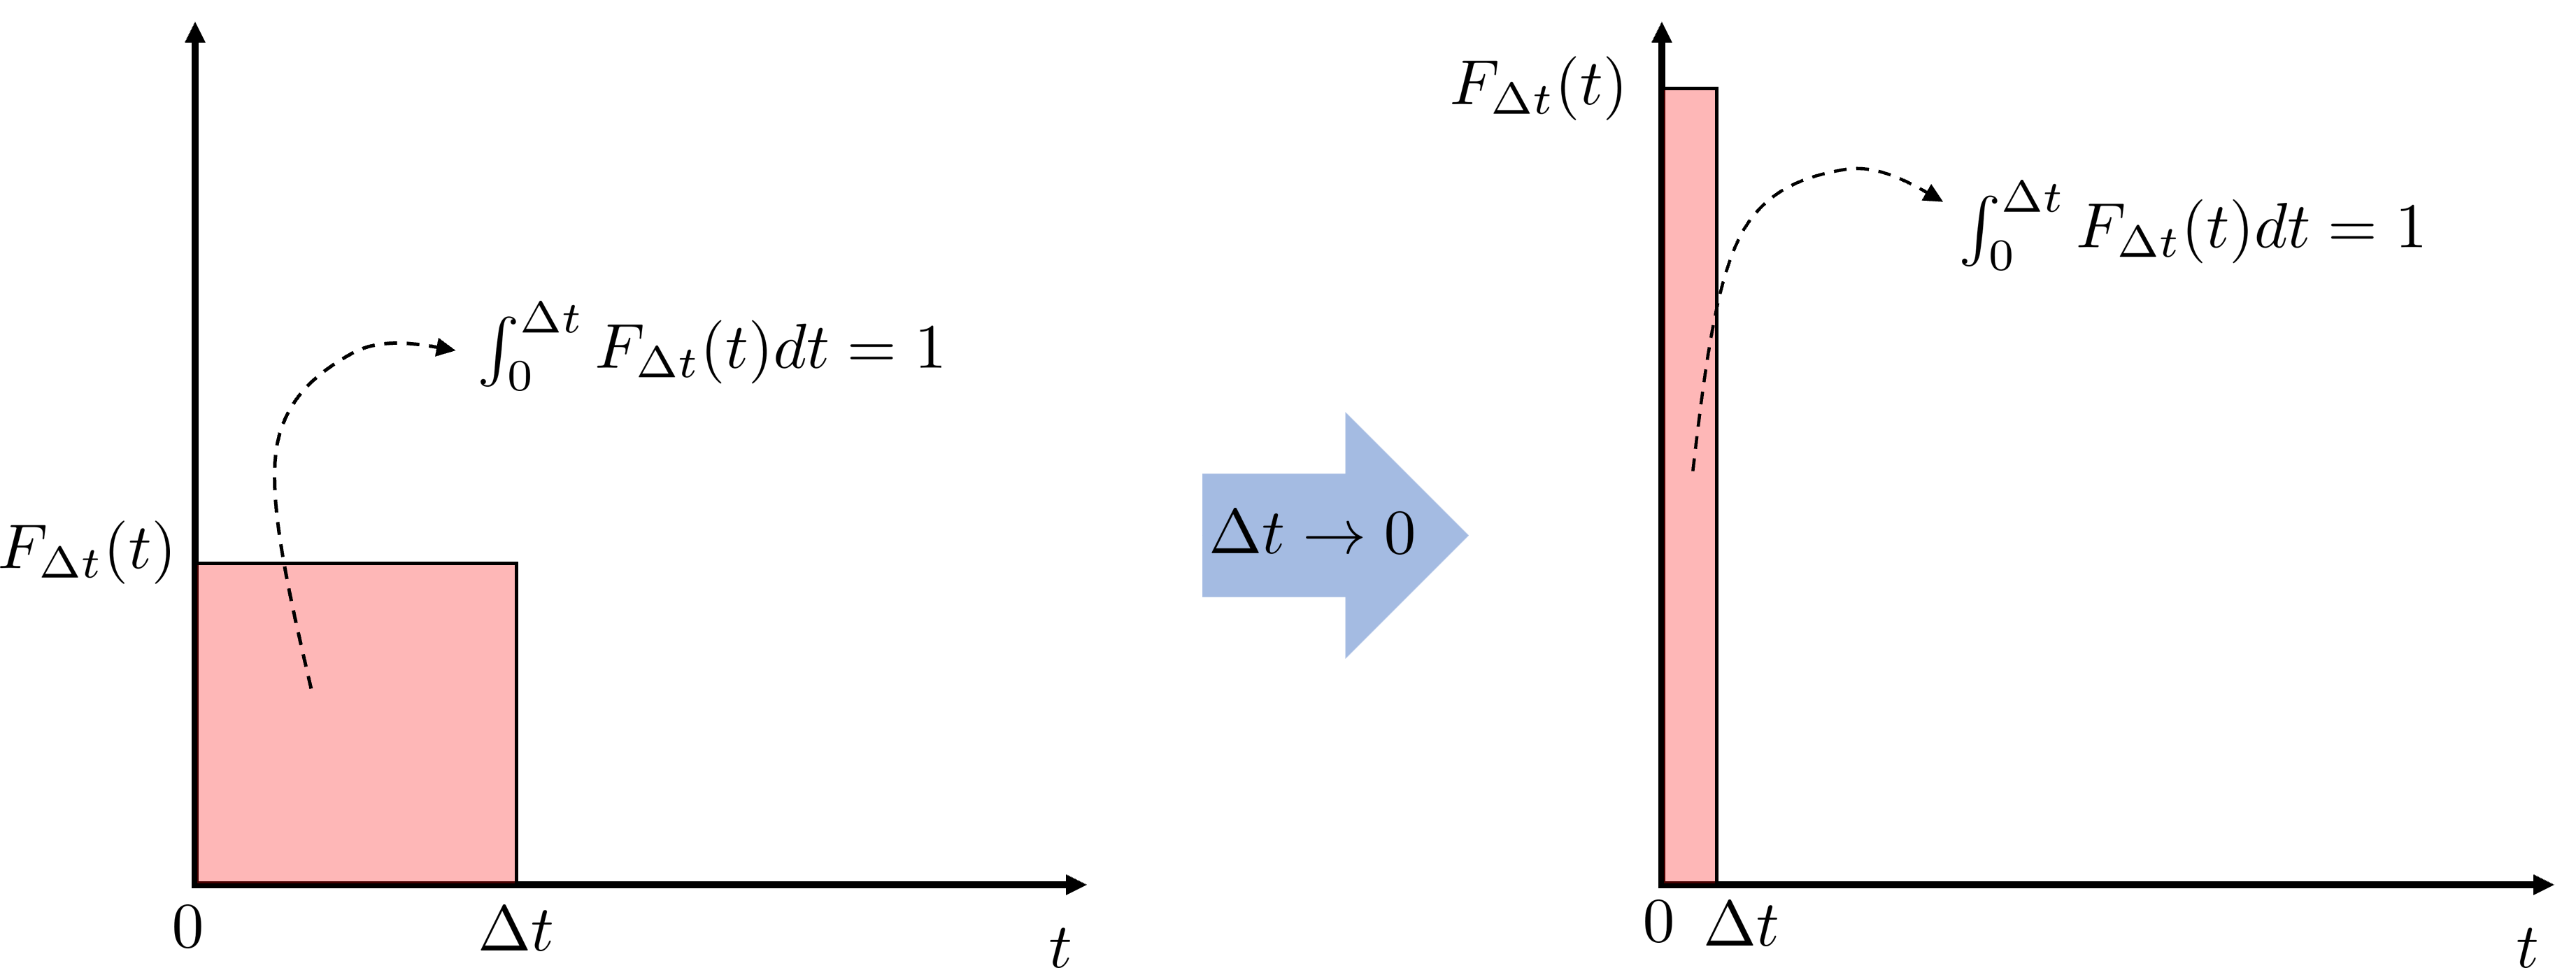
\includegraphics[width=20cm]{./FIG_Franklin/fig8-smc2.png}
	    \end{figure}

\end{enumerate}

